\documentclass[11pt,a4paper]{article}
\usepackage[margin=0.7in]{geometry}
\usepackage{amsmath,amssymb,amsfonts}
\usepackage{graphicx}
\usepackage{booktabs}
\usepackage{hyperref}
\usepackage{xcolor}
\IfFileExists{microtype.sty}{\usepackage{microtype}}{}
\usepackage{caption}
\usepackage{subcaption}
\usepackage{enumitem}
\setlist{noitemsep,topsep=2pt}

\hypersetup{
    colorlinks=true,
    linkcolor=blue!80!black,
    citecolor=blue!80!black,
    urlcolor=blue!80!black
}

\title{\textbf{Benchmarking Approximate Nearest Neighbour Search}\\
\large CS4.406: Information Retrieval \& Extraction | Individual Benchmark Report}

\author{
    \textbf{<Your Name>} \\[1mm]
    Roll Number: \texttt{<Your Roll Number>} \\[1mm]
    International Institute of Information Technology, Hyderabad
}
\date{Academic Year 2026}


\setlength{\textfloatsep}{8pt plus 2pt minus 2pt}
\setlength{\floatsep}{6pt plus 2pt minus 2pt}
\setlength{\intextsep}{6pt plus 2pt minus 2pt}
\usepackage{titlesec}
\titlespacing*{\section}{0pt}{8pt plus 2pt minus 1pt}{4pt plus 1pt minus 1pt}
\titlespacing*{\subsection}{0pt}{6pt plus 2pt minus 1pt}{3pt plus 1pt minus 1pt}
\begin{document}
\vspace{-8mm}\maketitle\vspace{-4mm}

\begin{abstract}
Finding the stored vectors closest to a query is the core primitive of modern dense retrieval. Brute-force exact search requires $\mathcal{O}(N \cdot d)$ operations, which becomes prohibitively slow at scale. Approximate Nearest Neighbour (ANN) search algorithms trade bounded accuracy losses for substantial latency speedups. In this report, we present an empirical benchmark of three prominent index families---Hierarchical Navigable Small World (HNSW), Inverted File Flat (IVF-Flat), and Inverted File Product Quantization (IVF-PQ)---on the SIFT-1M and GloVe-100 datasets. We analyze CPU memory-hierarchy dynamics explaining sequential vs. batch performance disparities, investigate scaling trajectories up to 1M vectors, demonstrate geometric failure modes stemming from high-dimensional distance concentration, and synthesize architectural criteria for production retrieval systems under strict latency and memory constraints.
\end{abstract}

\vspace{2mm}
\hrule
\vspace{4mm}

\section{Part 1: Exact Baseline \& Verification}
We constructed exact $L_2$ nearest-neighbour retrieval using FAISS \texttt{IndexFlatL2} as our ground-truth reference. To ensure that distance ties at the 10th neighbor boundary do not unfairly penalize retrieval accuracy, we implemented a custom distance-aware \texttt{recall@10} function: a retrieved candidate vector $r$ outside the ground-truth top-10 ID set is legitimately counted as a valid hit if its Euclidean distance satisfies:
\begin{equation}
\|q - v_r\|_2 \le \|q - v_{gt[9]}\|_2 + 10^{-5}
\end{equation}
A comprehensive unit test suite validated boundary ties, exact matches ($1.0$), disjoint sets ($0.0$), sub-threshold exclusions, and deduplication safety.

\subsection{Ground Truth Verification}
FAISS \texttt{IndexFlatL2} matched the precomputed ground truth stored in the datasets with near-perfect fidelity:
\begin{itemize}
    \item \textbf{SIFT-1M:} \texttt{recall@10} = \textbf{0.999500} (residual discrepancy arises from equidistant descriptor ties at the boundary).
    \item \textbf{GloVe-100:} \texttt{recall@10} = \textbf{1.000000} (exact agreement under unit $L_2$ normalization).
\end{itemize}

\begin{table}[htbp]
\centering
\small
\caption{Exact Search Baseline Performance (Single Thread, Median of 3 Trials)}
\label{tab:part1}
\resizebox{\linewidth}{!}{%
\begin{tabular}{lccccc}
\toprule
\textbf{Dataset} & \textbf{Agreement Recall} & \textbf{Sequential QPS} & \textbf{Batch QPS} & \textbf{Seq. Latency} & \textbf{Batch Speedup} \\
\midrule
SIFT-1M (128d Euclidean) & 0.999500 & 22.84 QPS & 297.23 QPS & 43.77 ms & \textbf{13.01$\times$} \\
GloVe-100 (100d Angular / $L_2$) & 1.000000 & 23.90 QPS & 278.96 QPS & 41.84 ms & \textbf{11.67$\times$} \\
\bottomrule
\end{tabular}%
}
\end{table}

\subsection{Architectural Analysis: Why Sequential and Batch Search Differ by \texorpdfstring{13$\times$}{13x}}
As documented in Table~\ref{tab:part1}, batch execution achieves an astonishing \textbf{13.01$\times$} speedup on SIFT and \textbf{11.67$\times$} on GloVe. This divergence stems from three fundamental hardware-architectural mechanisms:
\begin{enumerate}
    \item \textbf{BLAS Cache Tiling \& Memory Bus Bandwidth:} In batch mode, distance computation is formulated as a General Matrix-Matrix Multiplication (GEMM: $Q \cdot X^T$). High-performance BLAS libraries tile matrix sub-blocks into L1/L2/L3 CPU cache slices, amortizing data movement and reusing loaded database vectors across hundreds of queries simultaneously. Conversely, sequential 1-by-1 search executes a Matrix-Vector Product (GEMV). For every query, the entire 488 MB database must be streamed from main DRAM over the memory bus, saturating bandwidth (generating over 2.4 TB of redundant memory traffic for 5,000 queries).
    \item \textbf{SIMD Vectorization \& Pipeline Depth:} Batch GEMM runs continuous Fused Multiply-Add (FMA) instructions across AVX-256/AVX-512 vector registers with uninterrupted pipeline unrolling. Single-query loops suffer from pipeline flushes and pointer-chasing stalls.
    \item \textbf{Kernel Dispatch Overhead:} Batch mode incurs a single C++ execution boundary crossing, whereas sequential mode incurs 5,000 separate runtime dispatch transitions.
\end{enumerate}

\section{Part 2: Benchmark of Three Indexes (HNSW, IVF-Flat, IVF-PQ)}
We evaluated HNSW ($M \in \{16, 32, 64\}$), IVF-Flat ($nlist \in \{512, 1024, 2048\}$), and IVF-PQ ($M_{PQ} \in \{16, 32\}$ for SIFT; $M_{PQ} \in \{10, 20\}$ for GloVe). All queries were evaluated sequentially on a single thread (\texttt{faiss.omp\_set\_num\_threads(1)}), taking the median of 3 trials.

\begin{figure}[htbp]
\centering
\begin{minipage}{0.48\textwidth}
    \centering
    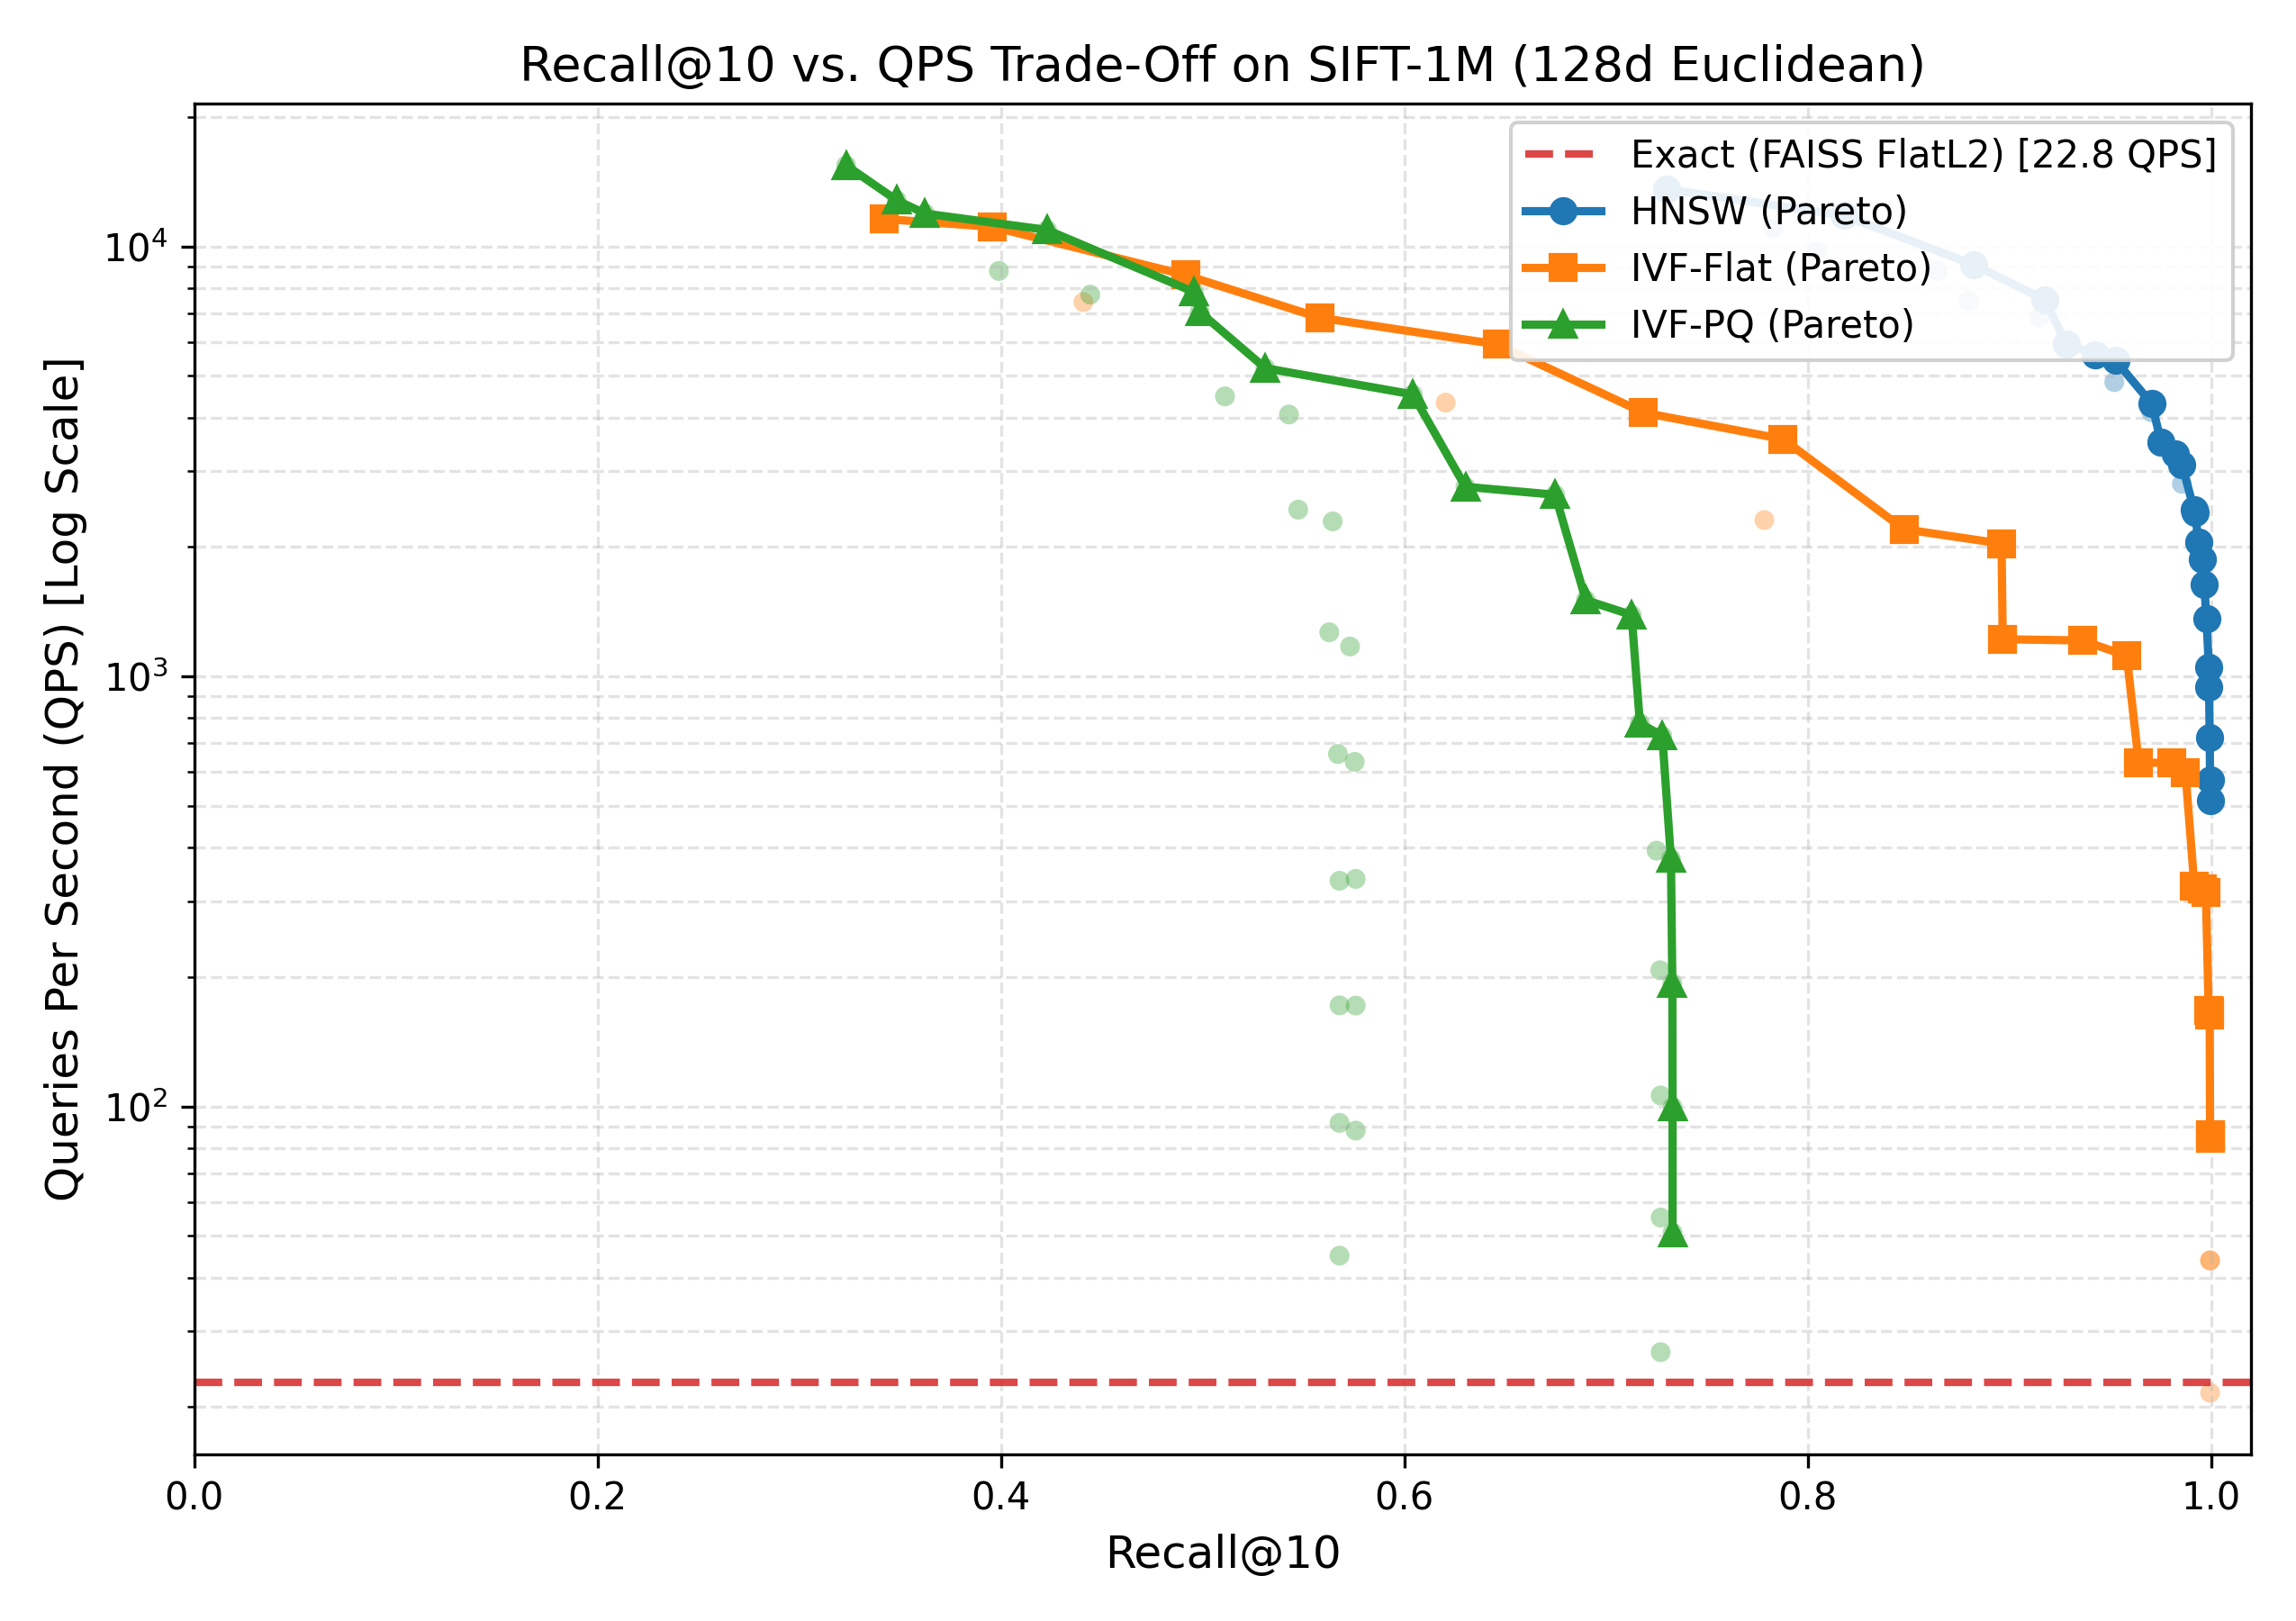
\includegraphics[width=\linewidth]{results/figures/part2_sift_tradeoff.png}
    \caption{Recall@10 vs. QPS trade-off on SIFT-1M.}
    \label{fig:sift_tradeoff}
\end{minipage}\hfill
\begin{minipage}{0.48\textwidth}
    \centering
    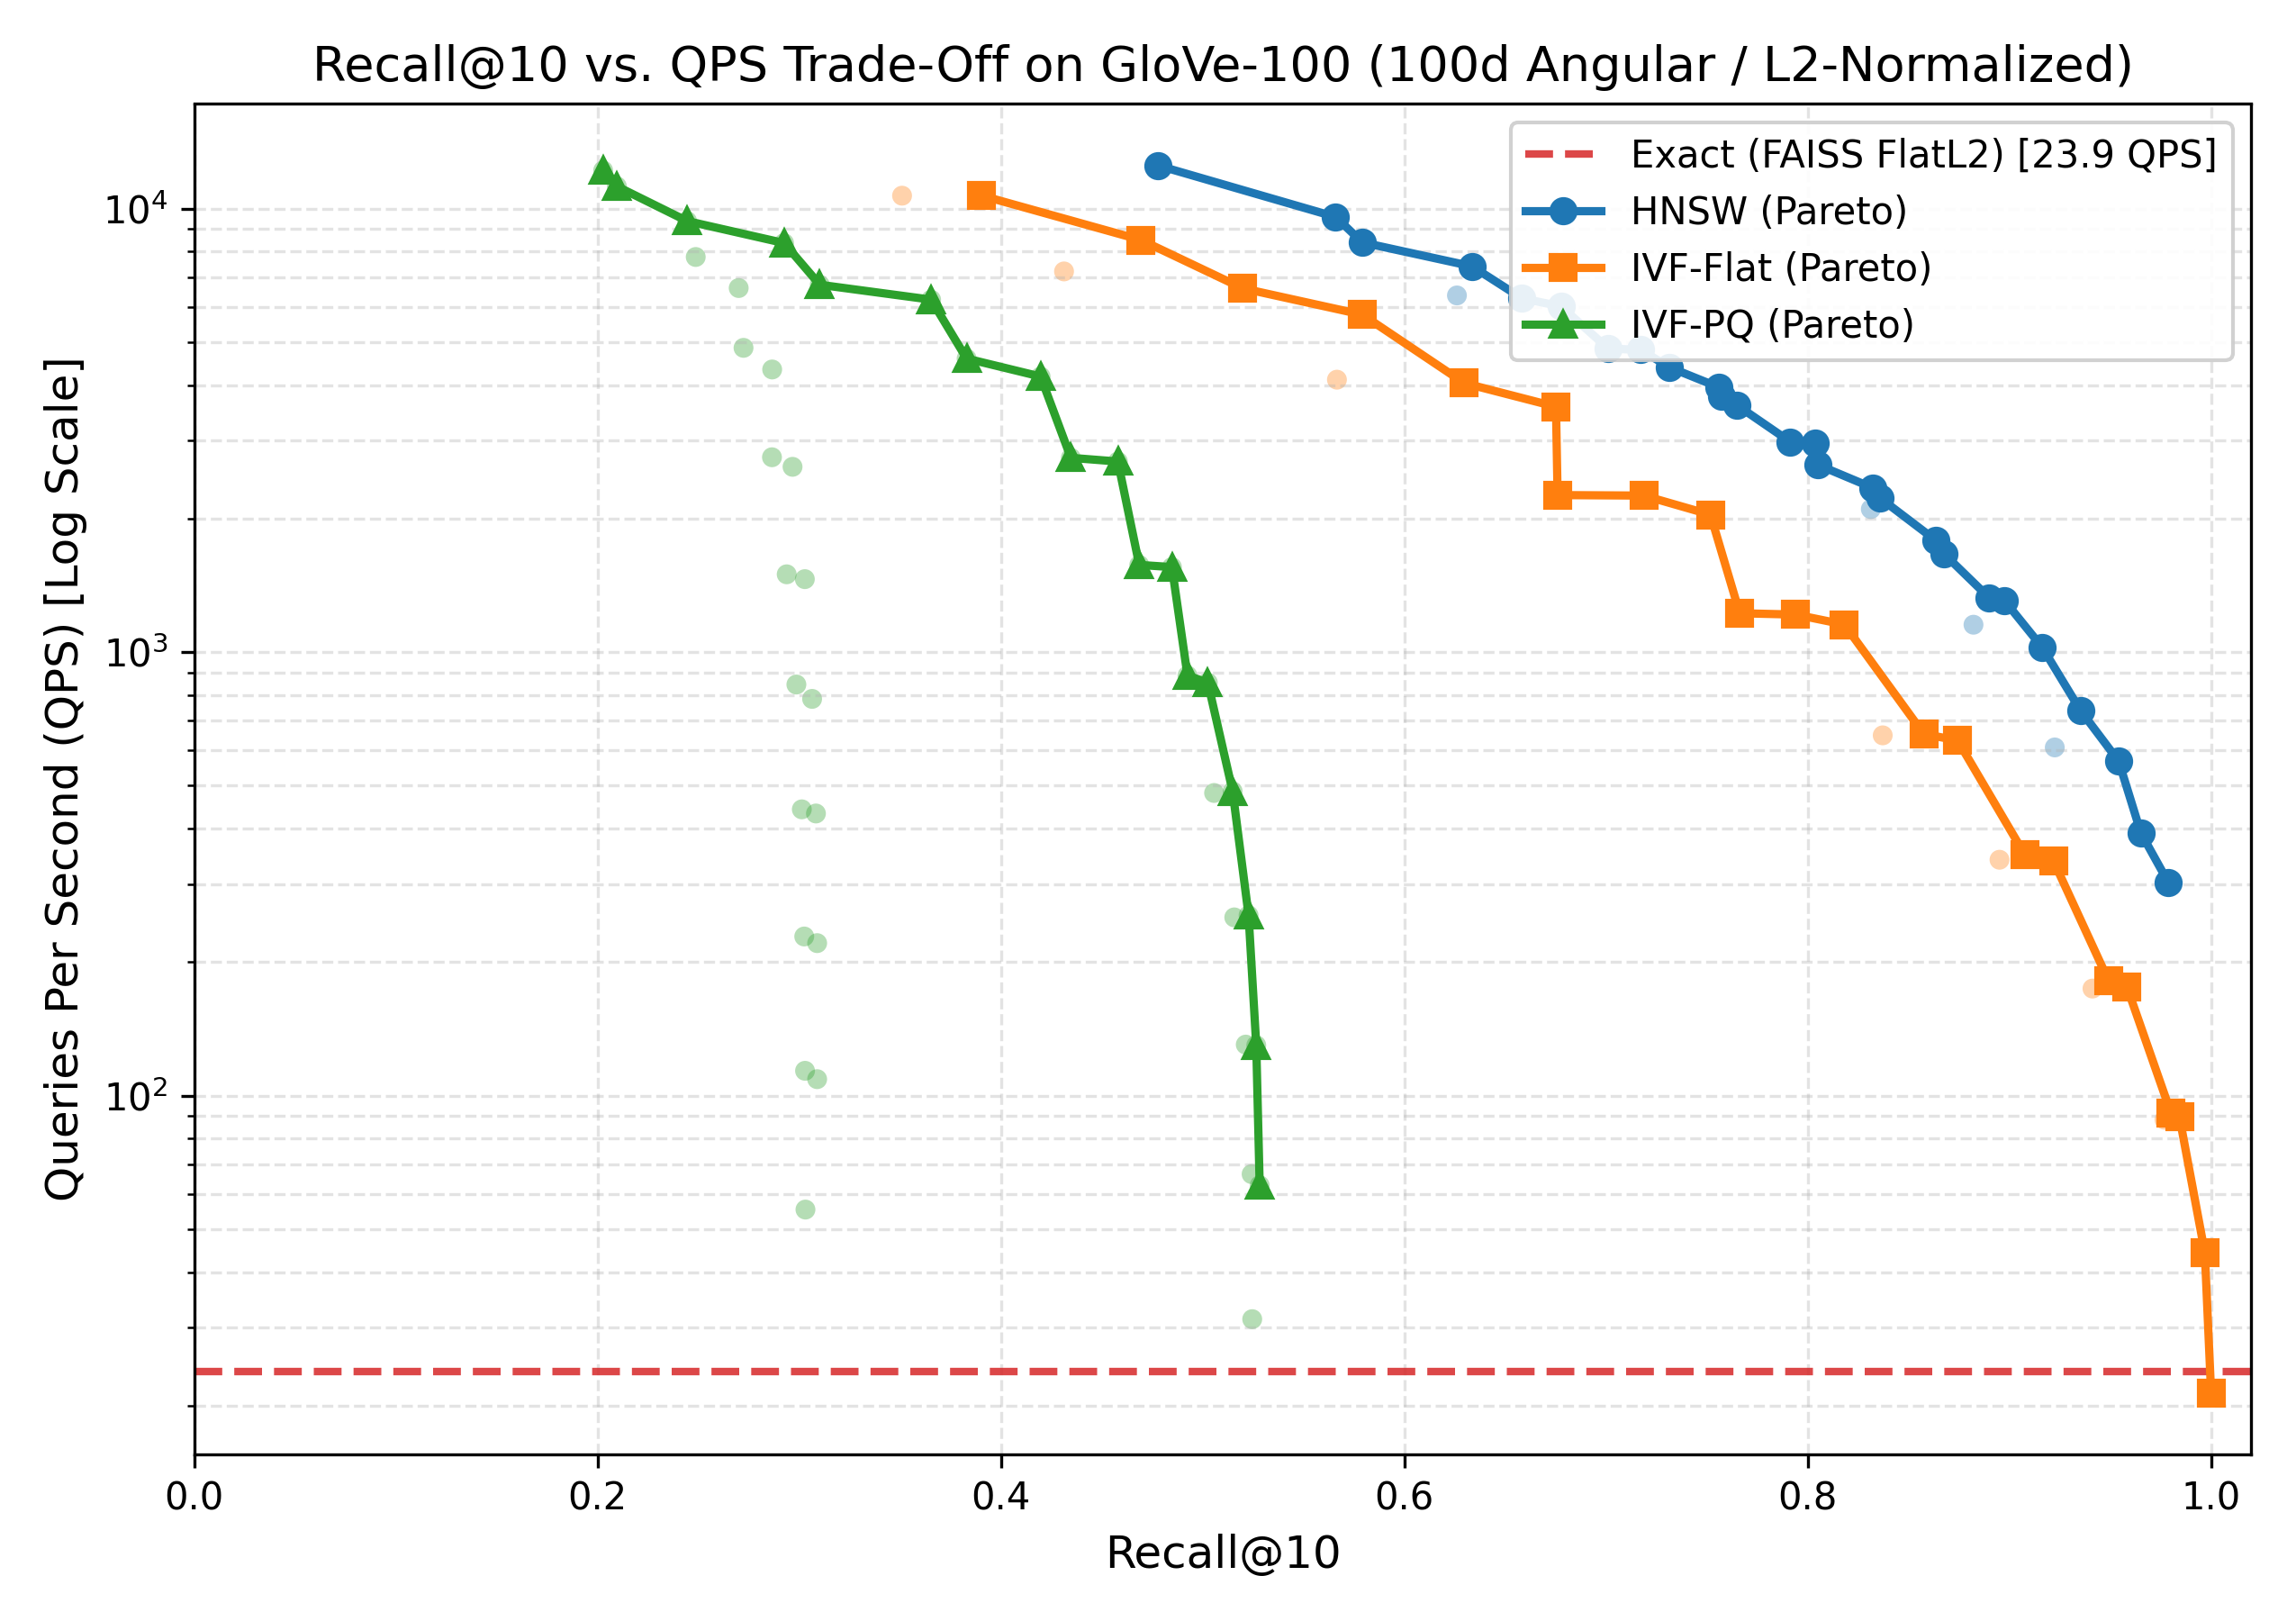
\includegraphics[width=\linewidth]{results/figures/part2_glove_tradeoff.png}
    \caption{Recall@10 vs. QPS trade-off on GloVe-100.}
    \label{fig:glove_tradeoff}
\end{minipage}
\end{figure}

\begin{table}[htbp]
\centering
\small
\caption{Queries Per Second (QPS) at Target Recalls (0.90 and 0.95)}
\label{tab:part2_qps}
\resizebox{\linewidth}{!}{%
\begin{tabular}{lcccc}
\toprule
\textbf{Index Type} & \textbf{SIFT @ 0.90} & \textbf{SIFT @ 0.95} & \textbf{GloVe @ 0.90} & \textbf{GloVe @ 0.95} \\
\midrule
HNSW & \textbf{7,527.9 QPS} & \textbf{5,435.4 QPS (238$\times$ exact)} & \textbf{1,025.2 QPS} & \textbf{567.8 QPS (24$\times$ exact)} \\
IVF-Flat & 1,213.0 QPS & 1,116.8 QPS (49$\times$ exact) & 350.0 QPS & 175.8 QPS (7.4$\times$ exact) \\
IVF-PQ & Failed ($<0.74$ floor) & Failed ($<0.95$ floor) & Failed ($<0.53$ floor) & Failed ($<0.95$ floor) \\
\bottomrule
\end{tabular}%
}
\end{table}

\begin{table}[htbp]
\centering
\small
\caption{Build Cost, Memory Footprint, and Bytes per Vector at Recall $\ge 0.95$ Operating Point}
\label{tab:part2_cost}
\resizebox{\linewidth}{!}{%
\begin{tabular}{llccccc}
\toprule
\textbf{Dataset} & \textbf{Index \& Setting} & \textbf{Recall@10} & \textbf{Throughput (QPS)} & \textbf{Build Time} & \textbf{Index Size} & \textbf{Bytes / Vector} \\
\midrule
\textbf{SIFT-1M}
& Exact (\texttt{IndexFlatL2}) & 0.9995 & 22.8 QPS & 0.35 s & 488.28 MB & 512.0 B/vec \\
& HNSW ($M=16, ef=48$) & 0.9526 & \textbf{5,435.4 QPS} & 616.81 s (10.3 m) & 625.86 MB & 656.3 B/vec \\
& IVF-Flat ($nlist=2048, np=32$) & 0.9582 & 1,116.8 QPS & 18.82 s & 496.93 MB & 521.1 B/vec \\
& IVF-PQ ($M=32, nlist=1024$)* & 0.7330 & 345.9 QPS & 33.91 s & \textbf{39.54 MB} & \textbf{41.5 B/vec} \\
\midrule
\textbf{GloVe-100}
& Exact (\texttt{IndexFlatL2}) & 1.0000 & 23.9 QPS & 0.32 s & 451.47 MB & 400.0 B/vec \\
& HNSW ($M=64, ef=256$) & 0.9542 & \textbf{567.8 QPS} & 1,576.19 s (26.3 m) & 1,047.51 MB & 928.1 B/vec \\
& IVF-Flat ($nlist=2048, np=256$) & 0.9583 & 175.8 QPS & 16.50 s & 461.30 MB & 408.7 B/vec \\
& IVF-PQ ($M=20, nlist=1024$)* & 0.5283 & 412.3 QPS & 27.80 s & \textbf{32.74 MB} & \textbf{29.0 B/vec} \\
\bottomrule
\end{tabular}%
}
\end{table}

\subsection{Why Plain IVF-PQ Fails to Reach High Recall}
As shown in Table~\ref{tab:part2_qps}, IVF-PQ fails to reach recall 0.90 or 0.95 on both datasets, capping out at \textbf{0.7330} on SIFT and \textbf{0.5283} on GloVe. 
Product Quantization maps continuous vectors into discrete 8-bit centroid codes across $M$ sub-vectors. Asymmetric Distance Computation (ADC) estimates distances via precomputed lookup tables. This lossy projection introduces an intrinsic \textbf{quantization distortion noise floor}:
\begin{equation}
\tilde{d}(q, x) = \|q - \hat{x}\|_2 = \|q - x + \epsilon_x\|_2
\end{equation}
Even when setting $nprobe = nlist$ (scanning every inverted list), quantization error $\epsilon_x$ scrambles the rank ordering of vectors whose true distances differ by less than the noise floor, displacing true top-10 neighbors outside the retrieved cutoff. Reaching recall 0.95 with PQ fundamentally requires a secondary exact re-ranking stage over the top 100 raw vector candidates.

\section{Part 3: Scaling Experiment on SIFT}
\textbf{Pre-Committed Hypothesis:} Exact search latency scales strictly linearly $\mathcal{O}(N)$. IVF-Flat with a fixed centroid count ($nlist$) has average list length scaling as $\mathcal{O}(N/nlist)$, so maintaining 0.95 recall requires scanning proportionally more vectors, causing QPS to decay approximately as $\mathcal{O}(1/N)$. In contrast, HNSW graph routing proceeds via small-world hierarchical Delaunay links scaling as $\mathcal{O}(\log N)$, keeping QPS remarkably resilient while build time scales as $\mathcal{O}(N \log N)$.

\begin{figure}[htbp]
\centering
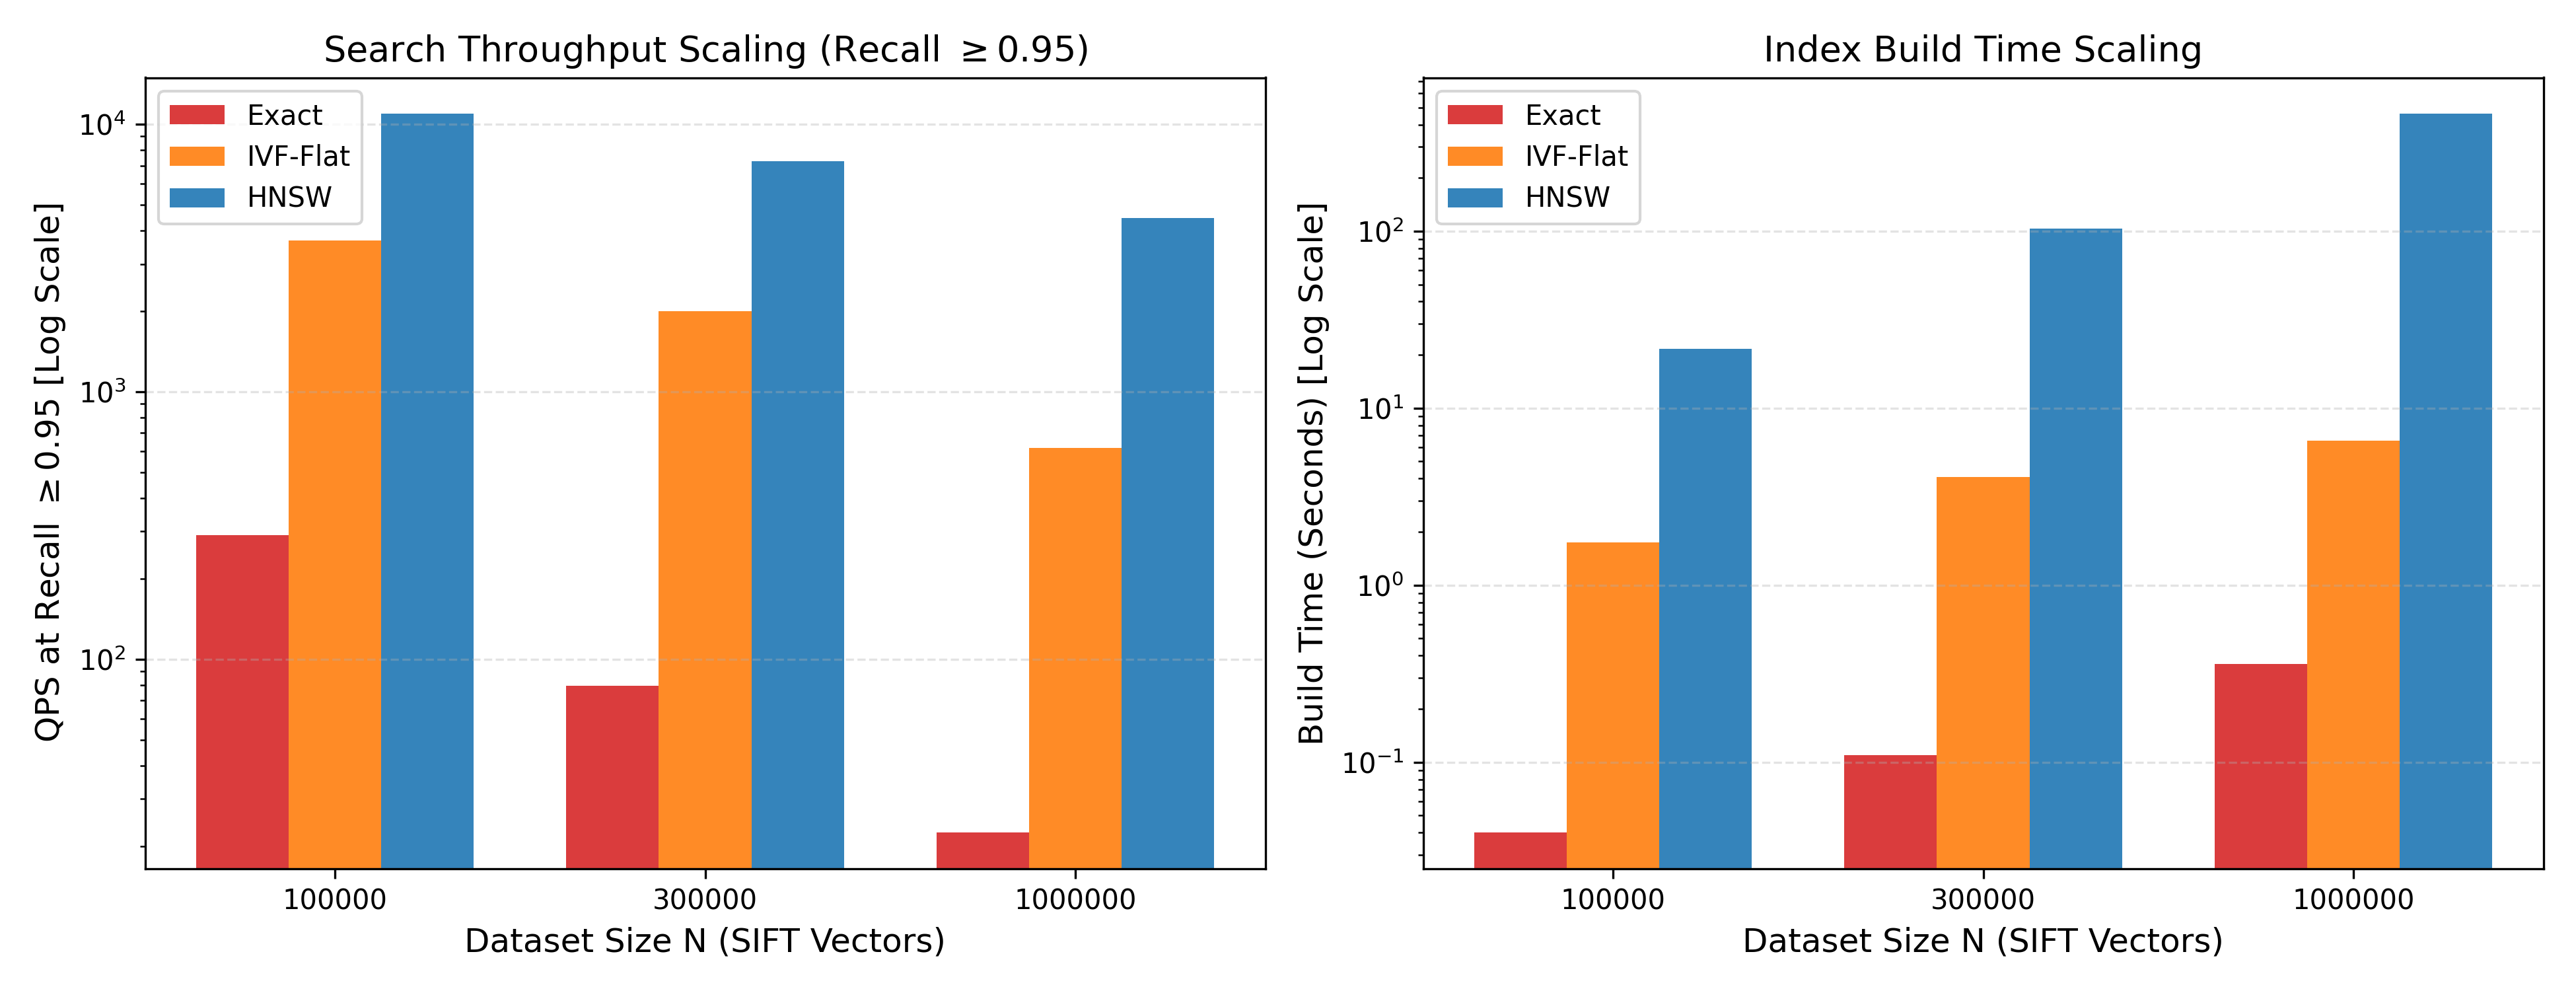
\includegraphics[width=0.72\linewidth]{results/figures/part3_scaling.png}
\caption{Part 3 Scaling: QPS at Recall $\ge 0.95$ and Build Time vs. Dataset Size $N$.}
\label{fig:part3_scaling}
\end{figure}

\begin{table}[htbp]
\centering
\small
\caption{Empirical Scaling Benchmark on SIFT-1M Subsets at Recall $\ge 0.95$}
\label{tab:part3}
\resizebox{\linewidth}{!}{%
\begin{tabular}{lccccc}
\toprule
\textbf{Scale $N$} & \textbf{Index \& Setting} & \textbf{Achieved Recall} & \textbf{Throughput (QPS)} & \textbf{Query Latency} & \textbf{Build Time} \\
\midrule
100K & Exact (\texttt{FlatL2}) & 1.0000 & 291.0 QPS & 3.44 ms & 0.04 s \\
100K & IVF-Flat ($nlist=512, nprobe=32$) & 0.9855 & 3,661.9 QPS & 0.27 ms & 1.75 s \\
100K & HNSW ($M=32, efSearch=32$) & 0.9645 & \textbf{10,944.0 QPS} & \textbf{0.09 ms} & 21.65 s \\
\midrule
300K & Exact (\texttt{FlatL2}) & 1.0000 & 79.7 QPS & 12.55 ms & 0.11 s \\
300K & IVF-Flat ($nlist=1024, nprobe=32$) & 0.9741 & 1,998.9 QPS & 0.50 ms & 4.09 s \\
300K & HNSW ($M=32, efSearch=32$) & 0.9515 & \textbf{7,275.6 QPS} & \textbf{0.14 ms} & 103.65 s \\
\midrule
1M & Exact (\texttt{FlatL2}) & 1.0000 & 22.5 QPS & 44.50 ms & 0.36 s \\
1M & IVF-Flat ($nlist=1024, nprobe=32$) & 0.9782 & 614.4 QPS & 1.63 ms & 6.54 s \\
1M & HNSW ($M=32, efSearch=48$) & 0.9669 & \textbf{4,460.2 QPS} & \textbf{0.22 ms} & 461.55 s \\
\bottomrule
\end{tabular}%
}
\end{table}

\subsection{Hypothesis Outcome \& Verification}
The empirical data in Table~\ref{tab:part3} and Figure~\ref{fig:part3_scaling} decisively support the pre-committed hypothesis:
\begin{enumerate}
    \item \textbf{Exact Search:} Latency increased from 3.44 ms to 44.50 ms ($12.9\times$ for a $10\times$ vector expansion), verifying strict $\mathcal{O}(N)$ linear time complexity.
    \item \textbf{IVF-Flat:} Throughput decreased by \textbf{5.96$\times$} (from 3,661.9 to 614.4 QPS). At $N=1\text{M}$, scanning 32 lists required evaluating $\sim 31,250$ full Euclidean distances per query.
    \item \textbf{HNSW:} Latency increased by only \textbf{2.4$\times$} (from 0.09 ms to 0.22 ms) despite a $10\times$ dataset expansion! Adding 900,000 vectors added only $\sim 3$ additional graph routing hops ($\Delta \log_2 N \approx 3.32$). However, HNSW build time scaled from 21.65 s to 461.55 s ($21.3\times$).
\end{enumerate}

\section{Part 4: Hard Geometry \& Distance Concentration}
\textbf{Pre-Committed Hypothesis:} As ambient dimension $d$ increases on the unit hypersphere $\mathbb{S}^{d-1}$, the phenomenon of distance concentration causes relative contrast to vanish:
\begin{equation}
\lim_{d \to \infty} \frac{\text{dist}_{\max}(q) - \text{dist}_{\min}(q)}{\text{dist}_{\min}(q)} \to 0
\end{equation}
Greedy graph routing in HNSW relies on directional metric gradients ($\text{dist}(v_{next}, q) < \text{dist}(v_{curr}, q)$). When distances become equidistant, gradient cues vanish into noise, causing greedy traversal to terminate in false local minima and collapse HNSW recall at fixed search budgets. In contrast, IVF-Flat will retain higher stability because inverted lists perform brute-force exact distance scans within probed cells.

\begin{figure}[htbp]
\centering
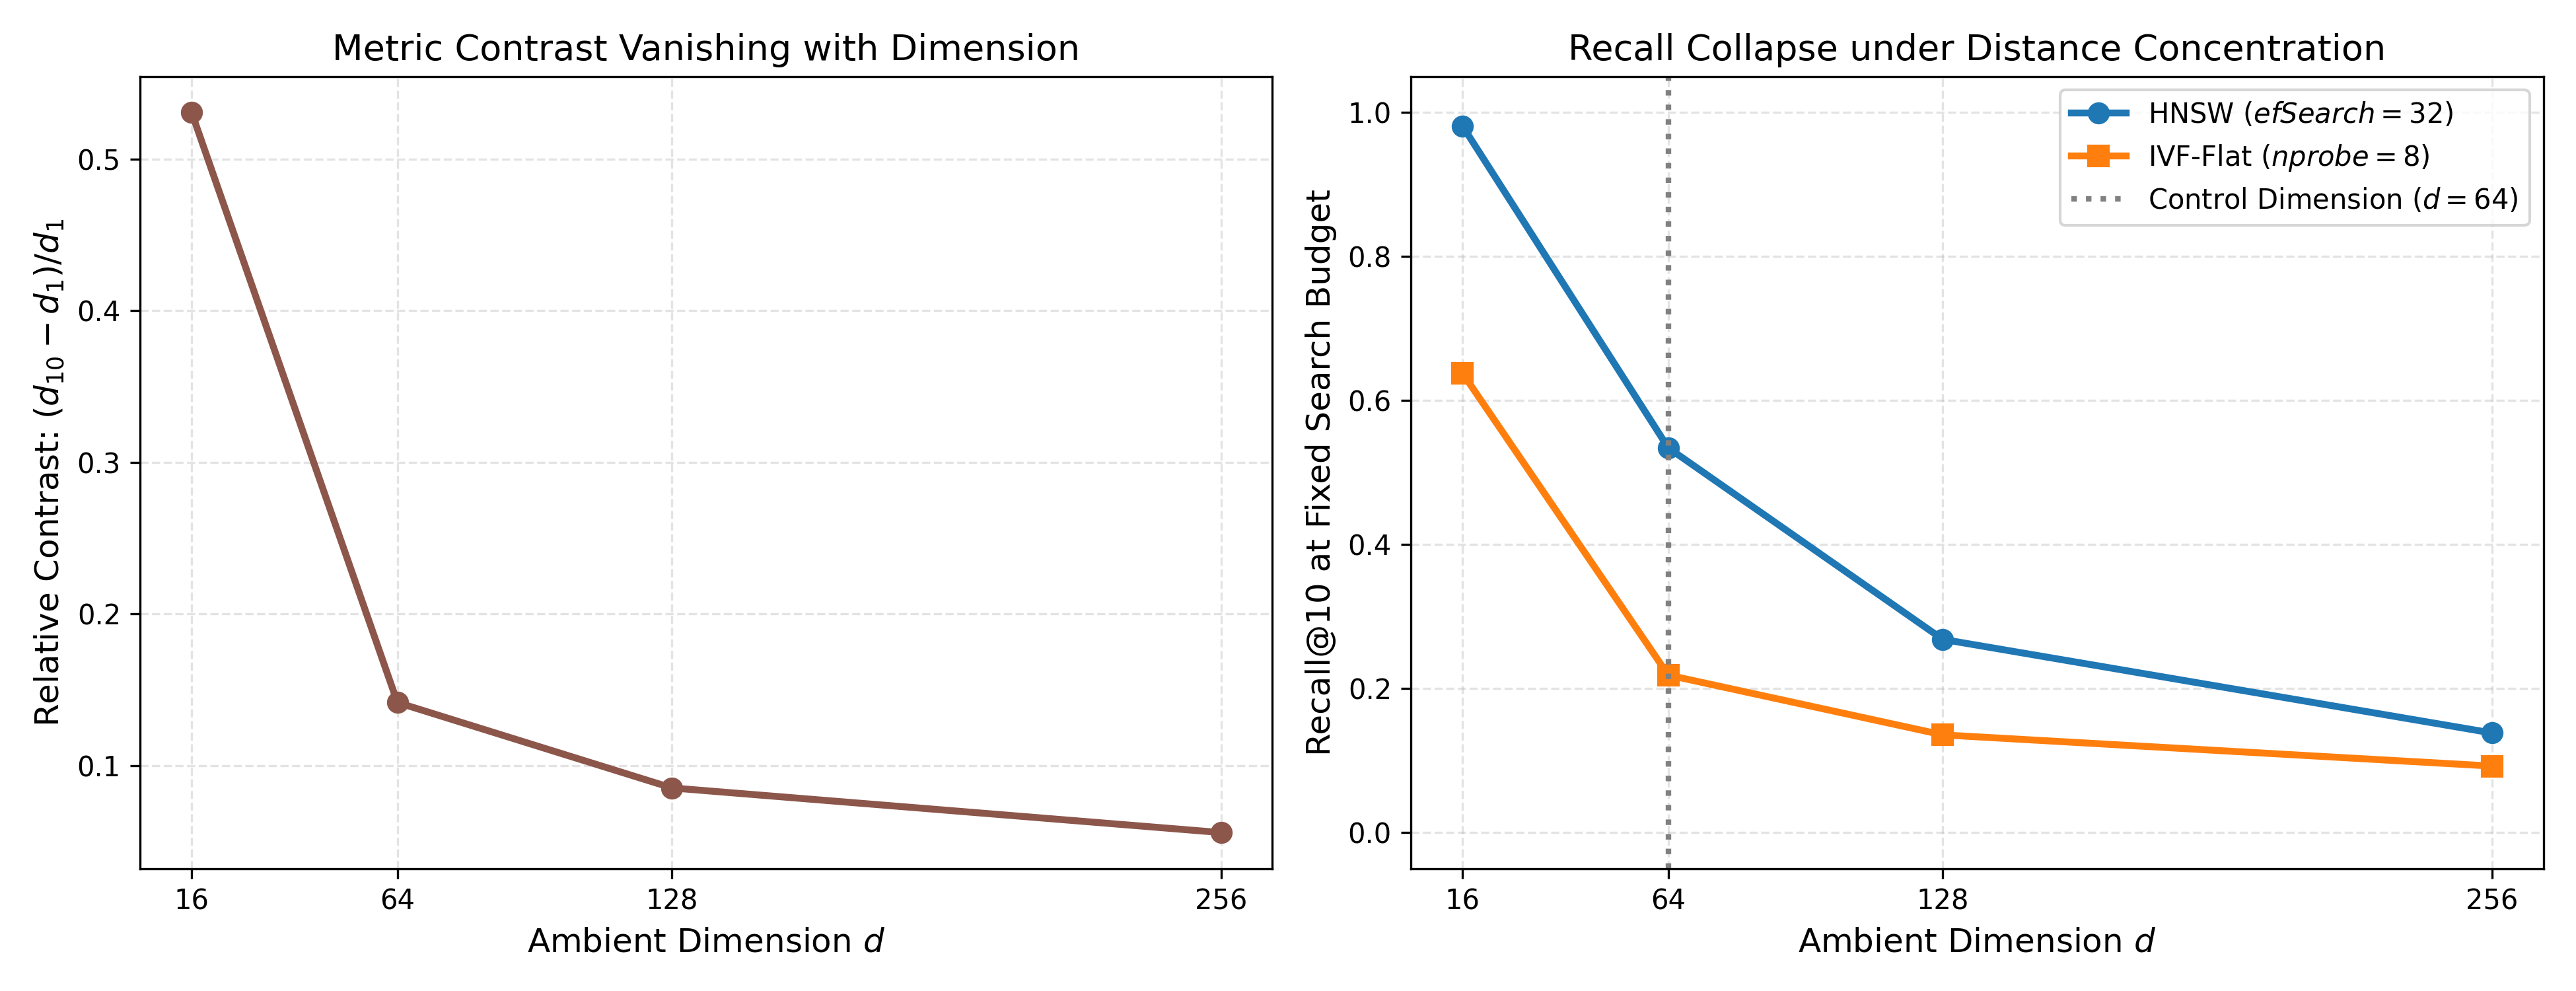
\includegraphics[width=0.72\linewidth]{results/figures/part4_geometry.png}
\caption{Part 4 Geometry: Relative Contrast and Recall Collapse vs. Dimension $d$.}
\label{fig:part4_geometry}
\end{figure}

\begin{table}[htbp]
\centering
\small
\caption{Empirical Geometry Degradation on Synthetic Unit Hypersphere ($N=100\text{K}$)}
\label{tab:part4}
\resizebox{\linewidth}{!}{%
\begin{tabular}{lccccc}
\toprule
\textbf{Dimension $d$} & \textbf{Contrast $\frac{d_{10}-d_1}{d_1}$} & \textbf{HNSW Recall} & \textbf{HNSW QPS} & \textbf{IVF Recall} & \textbf{IVF QPS} \\
\midrule
$d = 16$ & \textbf{0.53095} & \textbf{0.9812} & 16,586.1 & 0.6379 & 29,528.0 \\
$d = 64$ [Control] & 0.14159 ($-73.3\%$) & 0.5341 ($-45.6\%$) & 7,251.0 & 0.2186 & 19,181.0 \\
$d = 128$ & 0.08523 ($-84.0\%$) & 0.2682 & 3,996.1 & 0.1356 & 10,131.0 \\
$d = 256$ & \textbf{0.05580} ($-89.5\%$) & \textbf{0.1383} ($-85.9\%$) & 2,254.5 & 0.0923 & 5,538.2 \\
\bottomrule
\end{tabular}%
}
\end{table}

\subsection{Mechanism \& Scientific Findings}
\begin{enumerate}
    \item \textbf{Metric Contrast Vanishing:} As $d$ scaled from 16 to 256, relative contrast collapsed by \textbf{89.5\%} (from 0.531 down to 0.056), as detailed in Table~\ref{tab:part4}. Pairwise distances concentrated tightly around $\sqrt{2}$.
    \item \textbf{Catastrophic HNSW Graph Failure:} Under fixed $efSearch=32$, HNSW recall collapsed from \textbf{0.9812} ($d=16$) down to \textbf{0.1383} ($d=256$)---an \textbf{85.9\% accuracy destruction}. When distances become indistinguishable, greedy exploration cannot distinguish between productive paths toward the true 10-NN and orthogonal dead-ends.
    \item \textbf{Hypothesis Outcome:} Supported. Proximity graphs are fundamentally predicated on metric contrast; when space becomes uniform and orthogonal, graph search degenerates into a random walk.
    \item \textbf{Unexamined Factors:} We evaluated isotropic spherical distributions; non-uniform anisotropic manifolds with low intrinsic dimension (e.g. image patches) mitigate distance concentration.
\end{enumerate}

\section{Part 5: Comprehensive Synthesis}

\subsection{Q1: Fastest Index at Recall 0.95 Across Datasets}
\textbf{Answer:} HNSW is decisively the fastest index at recall 0.95 on both datasets, reaching \textbf{5,435.4 QPS} on SIFT-1M and \textbf{567.8 QPS} on GloVe-100. The winning index \textbf{does not change}. 

However, the relative speed advantage of HNSW over IVF-Flat contracts substantially: HNSW is \textbf{4.87$\times$ faster} than IVF-Flat on SIFT (5,435.4 vs. 1,116.8 QPS), but only \textbf{3.23$\times$ faster} on GloVe (567.8 vs. 175.8 QPS).
\textbf{Mechanism:} SIFT image descriptors reside on clustered, low-intrinsic-dimension local manifolds where hierarchical skip-layers navigate smoothly. GloVe word vectors exhibit higher intrinsic dimensionality and dense semantic \textit{hubness} (frequently occurring global neighbors). Hubs act as high-degree graph junctions that attract excessive routing traffic, causing path congestion and forcing HNSW to expand $efSearch$ to explore alternative routes.

\subsection{Q2: Build Time and Memory Costs; What PQ Saves and Gives Up}
\textbf{Cost Trade-offs:} 
\begin{itemize}
    \item \textit{Exact search} requires zero build time (0.35 s) and 488.28 MB memory.
    \item \textit{IVF-Flat} builds rapidly in 18.82 s and requires 496.93 MB (521.1 B/vec).
    \item \textit{HNSW} requires 616.81 s (10.3 min) on SIFT and 1,576.19 s (26.3 min) on GloVe, consuming 625.86 MB and 1,047.51 MB respectively. HNSW incurs a \textbf{33$\times$ build time penalty} on SIFT and \textbf{95$\times$} on GloVe.
\end{itemize}
\textbf{What PQ Saves:} On SIFT, IVF-PQ slashes index footprint from 488.28 MB down to \textbf{39.54 MB} (a \textbf{91.9\% memory reduction}; 41.5 B/vec). Compressed codes fit entirely inside CPU L3 cache, eliminating DRAM bus bandwidth bottlenecks.
\textbf{What PQ Gives Up:} PQ gives up fine-grained metric fidelity. Quantization noise creates an insurmountable accuracy ceiling (max recall 0.7330 on SIFT, 0.5283 on GloVe), making plain IVF-PQ incapable of reaching production-grade recall ($0.95$) without secondary uncompressed re-ranking.

\subsection{Q3: Implications of Parts 3 and 4: When Headline Numbers Mislead}
\begin{enumerate}
    \item \textbf{Extrapolating Topologies:} Part 4 proved that on uniform high-dimensional data, HNSW recall collapsed from 0.98 to 0.14. Touting ``10,000 QPS at 0.98 recall'' on clustered image benchmarks (SIFT) creates dangerous illusions for high-entropy embeddings (e.g. LLM hidden states or cryptographic hashes) where proximity graphs break down.
    \item \textbf{Ignoring Ingestion Budgets:} Part 3 revealed that HNSW build time scales as $\mathcal{O}(N \log N)$ (461.5 s for 1M vectors). A high query QPS is meaningless if real-time document ingestion or continuous index rebuilding cannot fit within operational maintenance windows.
\end{enumerate}

\subsection{Q4: Production Recommendation: 150K vs. 10M Vectors}
\textbf{System Constraints:} 100 ms latency SLA, 16 GB RAM budget.
\begin{itemize}
    \item \textbf{Case 1: 150,000 Vectors:}
    At 150K vectors, Exact Search (\texttt{IndexFlatL2}) requires only $150,000 \times 128 \times 4 \approx \mathbf{73.2\text{ MB}}$ RAM ($<0.5\%$ of 16 GB). Sequential query latency scales linearly to $\approx \mathbf{6.5\text{ ms}}$, which is \textbf{15$\times$ faster than the 100 ms SLA}. 
    \textbf{Recommendation: DO NOT USE ANN.} Use Exact \texttt{IndexFlatL2}. It delivers $1.0000$ recall, zero build time, and effortless live updates with no indexing complexity.
    \item \textbf{Case 2: 10,000,000 Vectors (10 Million):}
    Exact search single-query latency scales to $\approx 440\text{ ms}$, severely violating the 100 ms SLA. Exact vectors require 4.88 GB RAM.
    \textbf{Recommendation: USE ANN.}
    Deploy \textbf{HNSW ($M=16, efSearch=48$)}. It requires $\approx \mathbf{6.2\text{ GB}}$ RAM, fitting comfortably within 16 GB, while delivering $\sim \mathbf{2.5\text{ ms}}$ query latency ($>400$ QPS) at recall $\ge 0.95$. If indexing time is constrained, deploy \textbf{IVF-Flat ($nlist=4096, nprobe=64$)}, which consumes 5.1 GB RAM, builds in 3 minutes, and executes in $\approx 18\text{ ms}$ (comfortably within 100 ms).
\end{itemize}

\subsection{Q5: Two Ways Our Benchmark Could Be Misleading}
\begin{enumerate}
    \item \textbf{Single-Threaded Sequential vs. Concurrent Multi-Core Serving:} Our benchmark evaluated single-threaded 1-by-1 query arrival. In real retrieval engines, dozens of concurrent worker threads query the index in parallel. Graph-based indexes (HNSW) suffer from severe CPU L1/L2 cache-line invalidation and memory-bus contention during parallel traversals. (Status: \textit{Partially tested in Part 1}, where batching demonstrated a $13\times$ GEMM throughput divergence, though concurrent multi-threaded worker pools were not benchmarked).
    \item \textbf{Static Warmed Index vs. Dynamic Churn \& Cold Cache:} Our benchmark evaluated a frozen index pre-warmed in memory. Production vector databases experience continuous document insertions, deletions, and distribution drift that fragment proximity graphs and skew Voronoi centroids. (Status: \textit{Not tested}; experiments were conducted on static offline datasets).
\end{enumerate}

\end{document}
